%!TEX root = chi14grammatical.tex


The results imply that auto-suggest interfaces for syntactic search should show candidate relationships augmented with a list of phrases in which they occur. A list of phrases is the most recognizable presentation for clausal relationships (34\% beter than the baseline), and is as good as a list of words for the other types of relations. A mockup of such a search interface is shown in Figure \ref{fig:phrases-mockup}.  Selecting the choice will return all sentences that contain the search term and match the relation.
\begin{figure}
\centering
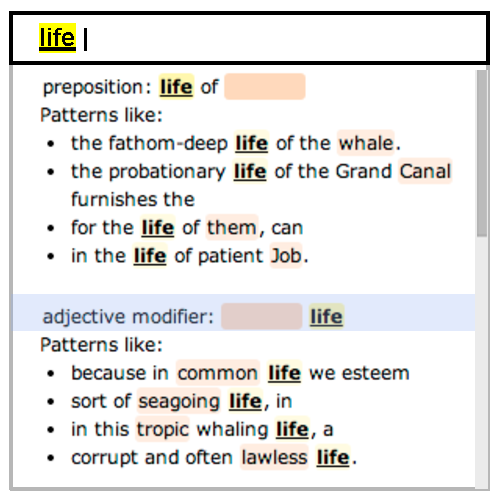
\includegraphics[width=0.5\columnwidth]{fig/phrases-mockup}
\caption{
	\label{fig:phrases-mockup} Mockup of auto-suggest for syntactic search on the word `seen', showing clausal relations with example phrases.
}
\end{figure}

There is a tradeoff between recognizability and space required for scrolling through the choices, although it is important to keep in mind that because the suggestions are populated with phrases from the collection itself, they are informative.    Further, the suggestions can be ordered by frequency of occurrence in the collection, or by an interestingness measure given the search word.  As the user becomes more familiar with a given relation, it may  be expedient to shorten the cues shown, and then re-introduce them if a relation has not been selected after some period of time as elapsed.

The best  strategy, \strong{phrases}, had an overall success rate of only 55\%, although the intended user base may have more familiarity with grammatical relations than the participants did, and therefore may perform better in practice.  Nonetheless, there is room for improvement in scores, and it may be that additional visual cues, such as some kind of bracketing, will improve results.  Furthermore, the current study did not test three-word relationships or more complex combinations of structures, and those may require improvements to the design.
